\chapter{Investigation}

\section{Applying Shannon's methods}
\textcite{Shannon1951} sets forth a method of analyzing the amount of information or uncertainty (i.e. entropy) each letter in an English text carries. In this section, I employ this method of analysis.

Shannon's approach in this paper builds on the concept of entropy as explained in \ref{subsec:shannon}. Rather than examining the entropy of individual letters out of context, he looks at the entropy of letters when the previous N-1 letters - the previous [N-1]-gram - is known. It formalizes the intuitive concept that there is more uncertainty when trying to guess a random letter in a text than there is when trying to guess a letter knowing its context.

To do this, he defines the sequences $G$ and $F$, where


$$G_n = -\sum_{b \in B_n} p(b) \log p(b)$$
$$F_n = G_n - G_{n-1} = -\sum_{b \in B_n} p(b) \log p(b)+\sum_{b \in B_{n-1}} p(b) \log p(b)$$

where $B_n$ is the set of all possible N-grams and $p(b)$ is the probability of a randomly chosen N-gram from an English text being equal to $b$.

$G_n$ is simply the entropy of N-grams. For example, $G_1 = p('e') log p('e') + p('t') log p('t') + ...$ is the entropy of 1-grams, that is, single letters.

$F_n$ is the differential or marginal entropy at the last letter of an N-gram, that is, how much uncertainty there is about that letter when the previous $n-1$ letters are known, and correspondingly how much information it carries.

To estimate these values for various values of $n$, I concatenate 97 texts obtained from Project Gutenberg and use python's \texttt{Counter} tool to count the number of occurrences of n-grams for various values of $n$. The results are shown in tables \ref{tab:n_gram_entropy} and \ref{tab:n_word_entropy}.


\begin{table}[h]
\centering
\begin{tabular}{ |p{1cm}||p{3cm}|p{3cm}|  }
 %\hline
 %\multicolumn{3}{|c|}{Compression algorithm benchmarks} \\
 \hline
    N  & N-gram entropy & Marginal entropy\\
 \hline
    1  &     4.674789   &      4.674789\\
    2  &     8.193527   &      3.518738\\
    3  &    11.077931   &      2.884403\\
    4  &    13.430718   &      2.352787\\
    5  &    15.434333   &      2.003615\\
    6  &    17.216262   &      1.781929\\
    7  &    18.825973   &      1.609712\\
    8  &    20.264030   &      1.438057\\
    9  &    21.517189   &      1.253159\\
    10 &    22.574182   &      1.056994\\
 \hline
\end{tabular}
\caption{Entropies and marginal entropies for substrings which are $n$ letters long
\label{tab:n_gram_entropy}}
\end{table}



\begin{table}[h]
\centering
\begin{tabular}{ |p{1cm}||p{3cm}|p{3cm}|  }
 %\hline
 %\multicolumn{3}{|c|}{Compression algorithm benchmarks} \\
 \hline
    N  & N-word entropy & Marginal entropy\\
 \hline
    1  &    11.477039   &     11.477039\\
    2  &    18.702746   &      7.225707\\
    3  &    22.187337   &      3.484592\\
    4  &    23.213621   &      1.026283\\
    5  &    23.434336   &      0.220715\\
    6  &    23.479111   &      0.044775\\
    7  &    23.491305   &      0.012193\\
    8  &    23.496988   &      0.005683\\
    9  &    23.500703   &      0.003715\\
    10 &    23.503611   &      0.002908\\
 \hline
\end{tabular}
\caption{Entropies and marginal entropies for substrings which are $n$ words long
\label{tab:n_word_entropy}}
\end{table}

Table \ref{tab:n_gram_entropy} shows the entropies for substrings of the text which are $n$ letters long, along with the entropy of the last letter, conditional on knowledge of the previous $n-1$ letters, while table \ref{tab:n_word_entropy} shows entropies for substrings which are $n$ words long, along with the entropy of the last word.

As can be seen in both tables, more knowledge about the context in which a letter or word appears decreases the information content and increases the predictability of that letter or word.




\section{Benchmarking compression algorithms}

For a rough bound on what's practically possible given common tools, I start by analyzing the performance of various existing non-text-specific compression algorithms on a collection of 97 texts in the public domain obtained from Project Gutenberg. The result of this benchmarking is displayed in table \ref{tab:compalg_benchmarks}.

\begin{table}[ht]
\centering
\begin{tabular}{ |p{3cm}||p{4cm}|p{3cm}|  }
 %\hline
 %\multicolumn{3}{|c|}{Compression algorithm benchmarks} \\
 \hline
 Algorithm & Compressed size (bytes) & Ratio\\
 \hline
    LZMA & 20815738 & 3.745084\\
    bzip2 & 21055590 & 3.702422\\
    gzip & 28702450 & 2.716029\\
    zlib & 28840353 & 2.703042\\
    No compression & 77956688 & 1.000000\\
 \hline
\end{tabular}
\caption{Compression algorithm benchmarks
\label{tab:compalg_benchmarks}}
\end{table}

The best performing compression algorithm is the Lempel–Ziv–Markov chain algorithm (LZMA), with a compression ratio of 3.745. Given that the vast majority of letters in Gutenberg texts are represented in a single byte (except for unicode characters), this compression method indicates that, at most, each byte in these texts contains on average 8/3.745 = 2.14 bits of entropy. We can expect compression methods which exploit more of the structure of natural language to push this closer to the theoretical limit.

\section{Co-compression}

As previously outlined, the theme of this project is the relationship between compression and comprehension. One point of commonality between these is the need for parsimony. This is expressed by Occam's razor, which states that "entities must not be multiplied beyond necessity" and commonly understood to mean that "the simplest explanation is usually the best one". 

Compression algorithms, for example the family of Lempel-Ziv algorithms, operate by eliminating the multiplication of entities through the creation of a codebook. If the relationship between compression and comprehension holds, we should expect to be able to use an existing compression algorithm like LZMA to get a rudimentary understanding of text.

\textcite{Jiang2023} showed that it's possible to use gzip for text classification, based on

\begin{displayquote}
"the intuitions that
\begin{enumerate}
\item compressors are good at capturing regularity; 
\item objects from the same category share more regularity than those from different categories"
\end{enumerate}
\end{displayquote}

To illustrate this using the same 97 Gutenberg texts mentioned earlier, I use the following scoring methods to estimate the similarity of a pair of texts:

\[add(y|x) = \frac{C(xy) - C(x)}{C(y)}\]

where \(C(t)\) is the compressed length of \(t\) expressed in bytes, \(xy\) is the concatenation of the texts \(x\) and \(y\). The function \(add(y|x)\) is then a measure of the additional information given by \(y\) when \(x\) is taken as a known basis.

To give an intuition for why the measure is defined in this way, it's helpful to use an example. Suppose that $x$ is the text of the complete works of Shakespeare and that $y$ is the text of Romeo and Juliet. Since $x$ contains $y$ as a substring, we should expect that a good compression algorithm would compress the concatenation $xy$ in little more space than is required for just $x$, as the entire text of $y$ can be signified with a symbol in the codebook, compressed once, and referred to twice.

Because of this, we should expect the value of $add(y|x)$ in this case to be close to 0, corresponding to the fact that $y$ does not really add information to $x$. Conversely, since the complete works of Shakespeare contain a lot of information not contained in just Romeo and Juliet, we should expect $add(x|y)$ to be close to 1, indicating that our compression algorithm's knowledge of the text of Romeo and Juliet only makes a small dent in the number of additional bits it needs to represent the works of Shakespeare.

The measure used above contrasts with Normalized Compression Distance (NCD) as used by \textcite{li2004similarity} , in that it is directional, i.e. that \(add(x|y)\) is not necessarily equal to \(add(y|x)\).

We may also define a more intuitive similarity score as follows

\[similarity(y|x) = 1 - add(y|x) = \frac{C(x) + C(y) - C(xy)}{C(y)}\]

This score giving a measure of the similarity of \(y\) to \(x\). In this case, $similarity(a|b)=1$ would indicate that $a$ is fully described by $b$ (as it contains no additional information), and $similarity(a|b)=0$ indicates that $a$ is unlike anything seen in $b$. Again, note that \(similarity(y|x)\) is not necessarily equal to \(similarity(x|y)\).

\begin{figure}[t]
\centering
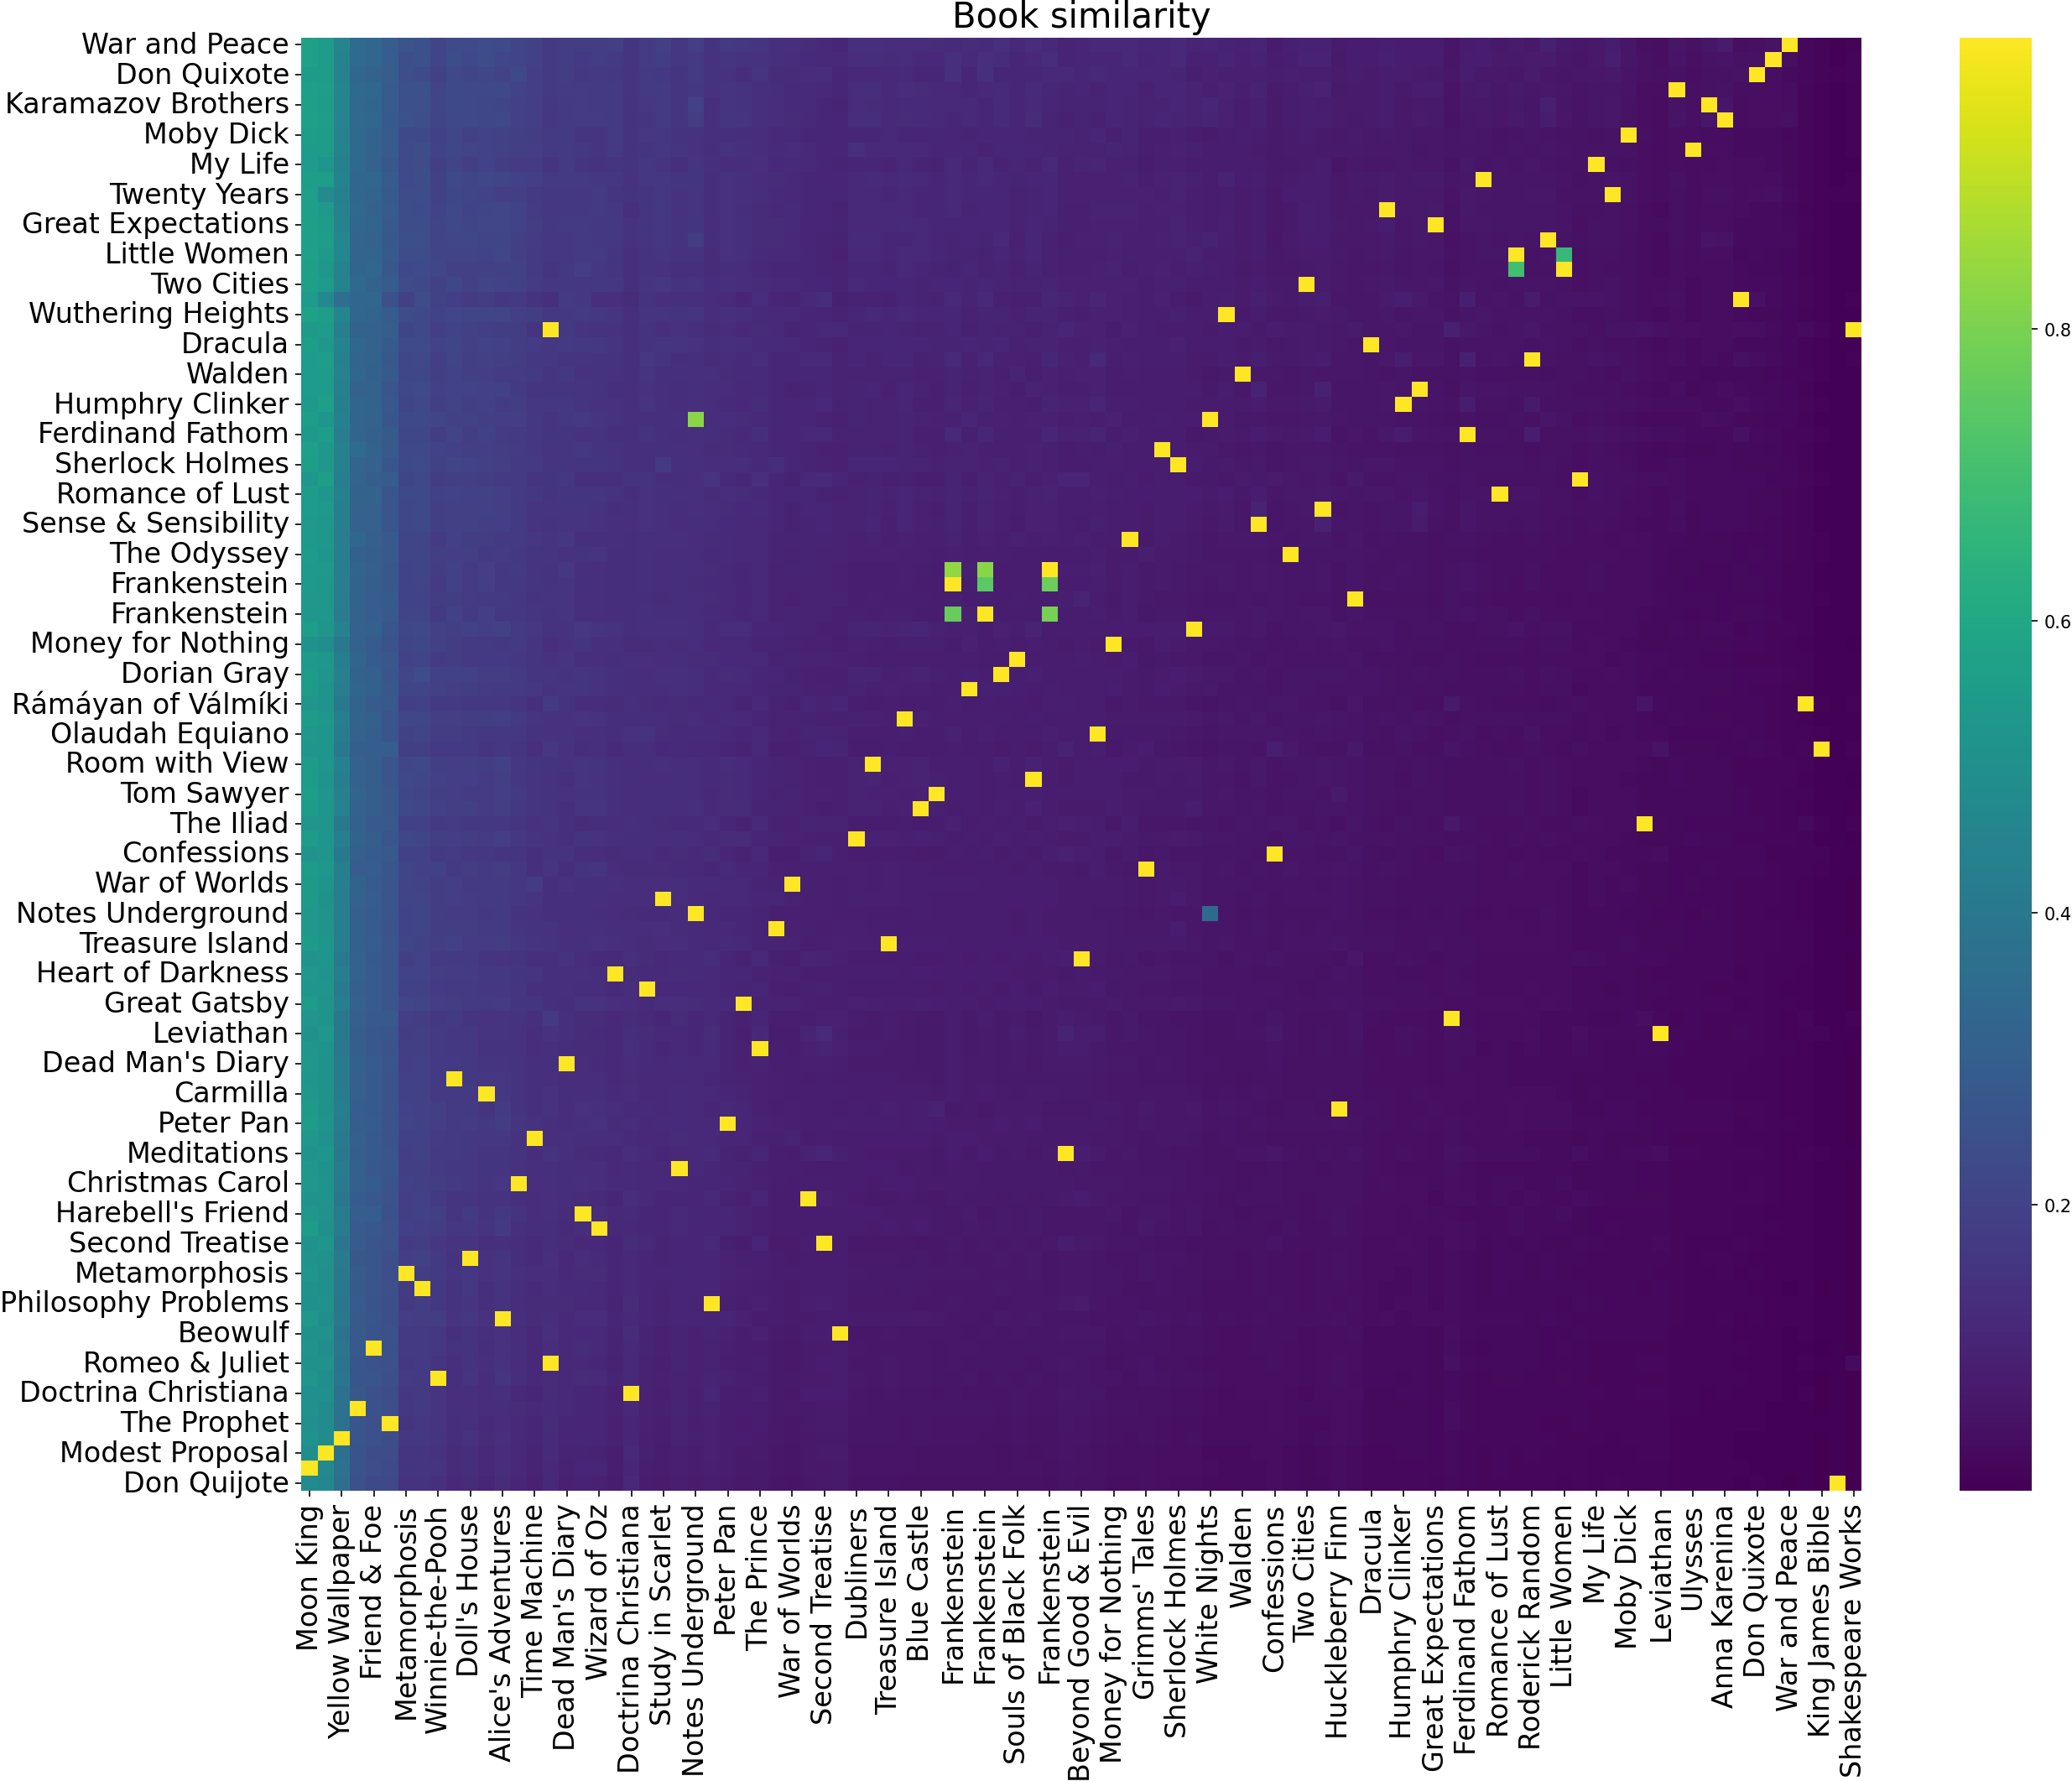
\includegraphics[width=\textwidth]{img/fig_co-compression_median.png}
\caption{Similarity scores for pairs of texts. The texts on the vertical axis are ordered most-predictive-first, and those on the horizontal axis are ordered most-predictable-first.}
\label{fig:heatmap_ppsort}
\end{figure}

\begin{figure}[t]
\centering
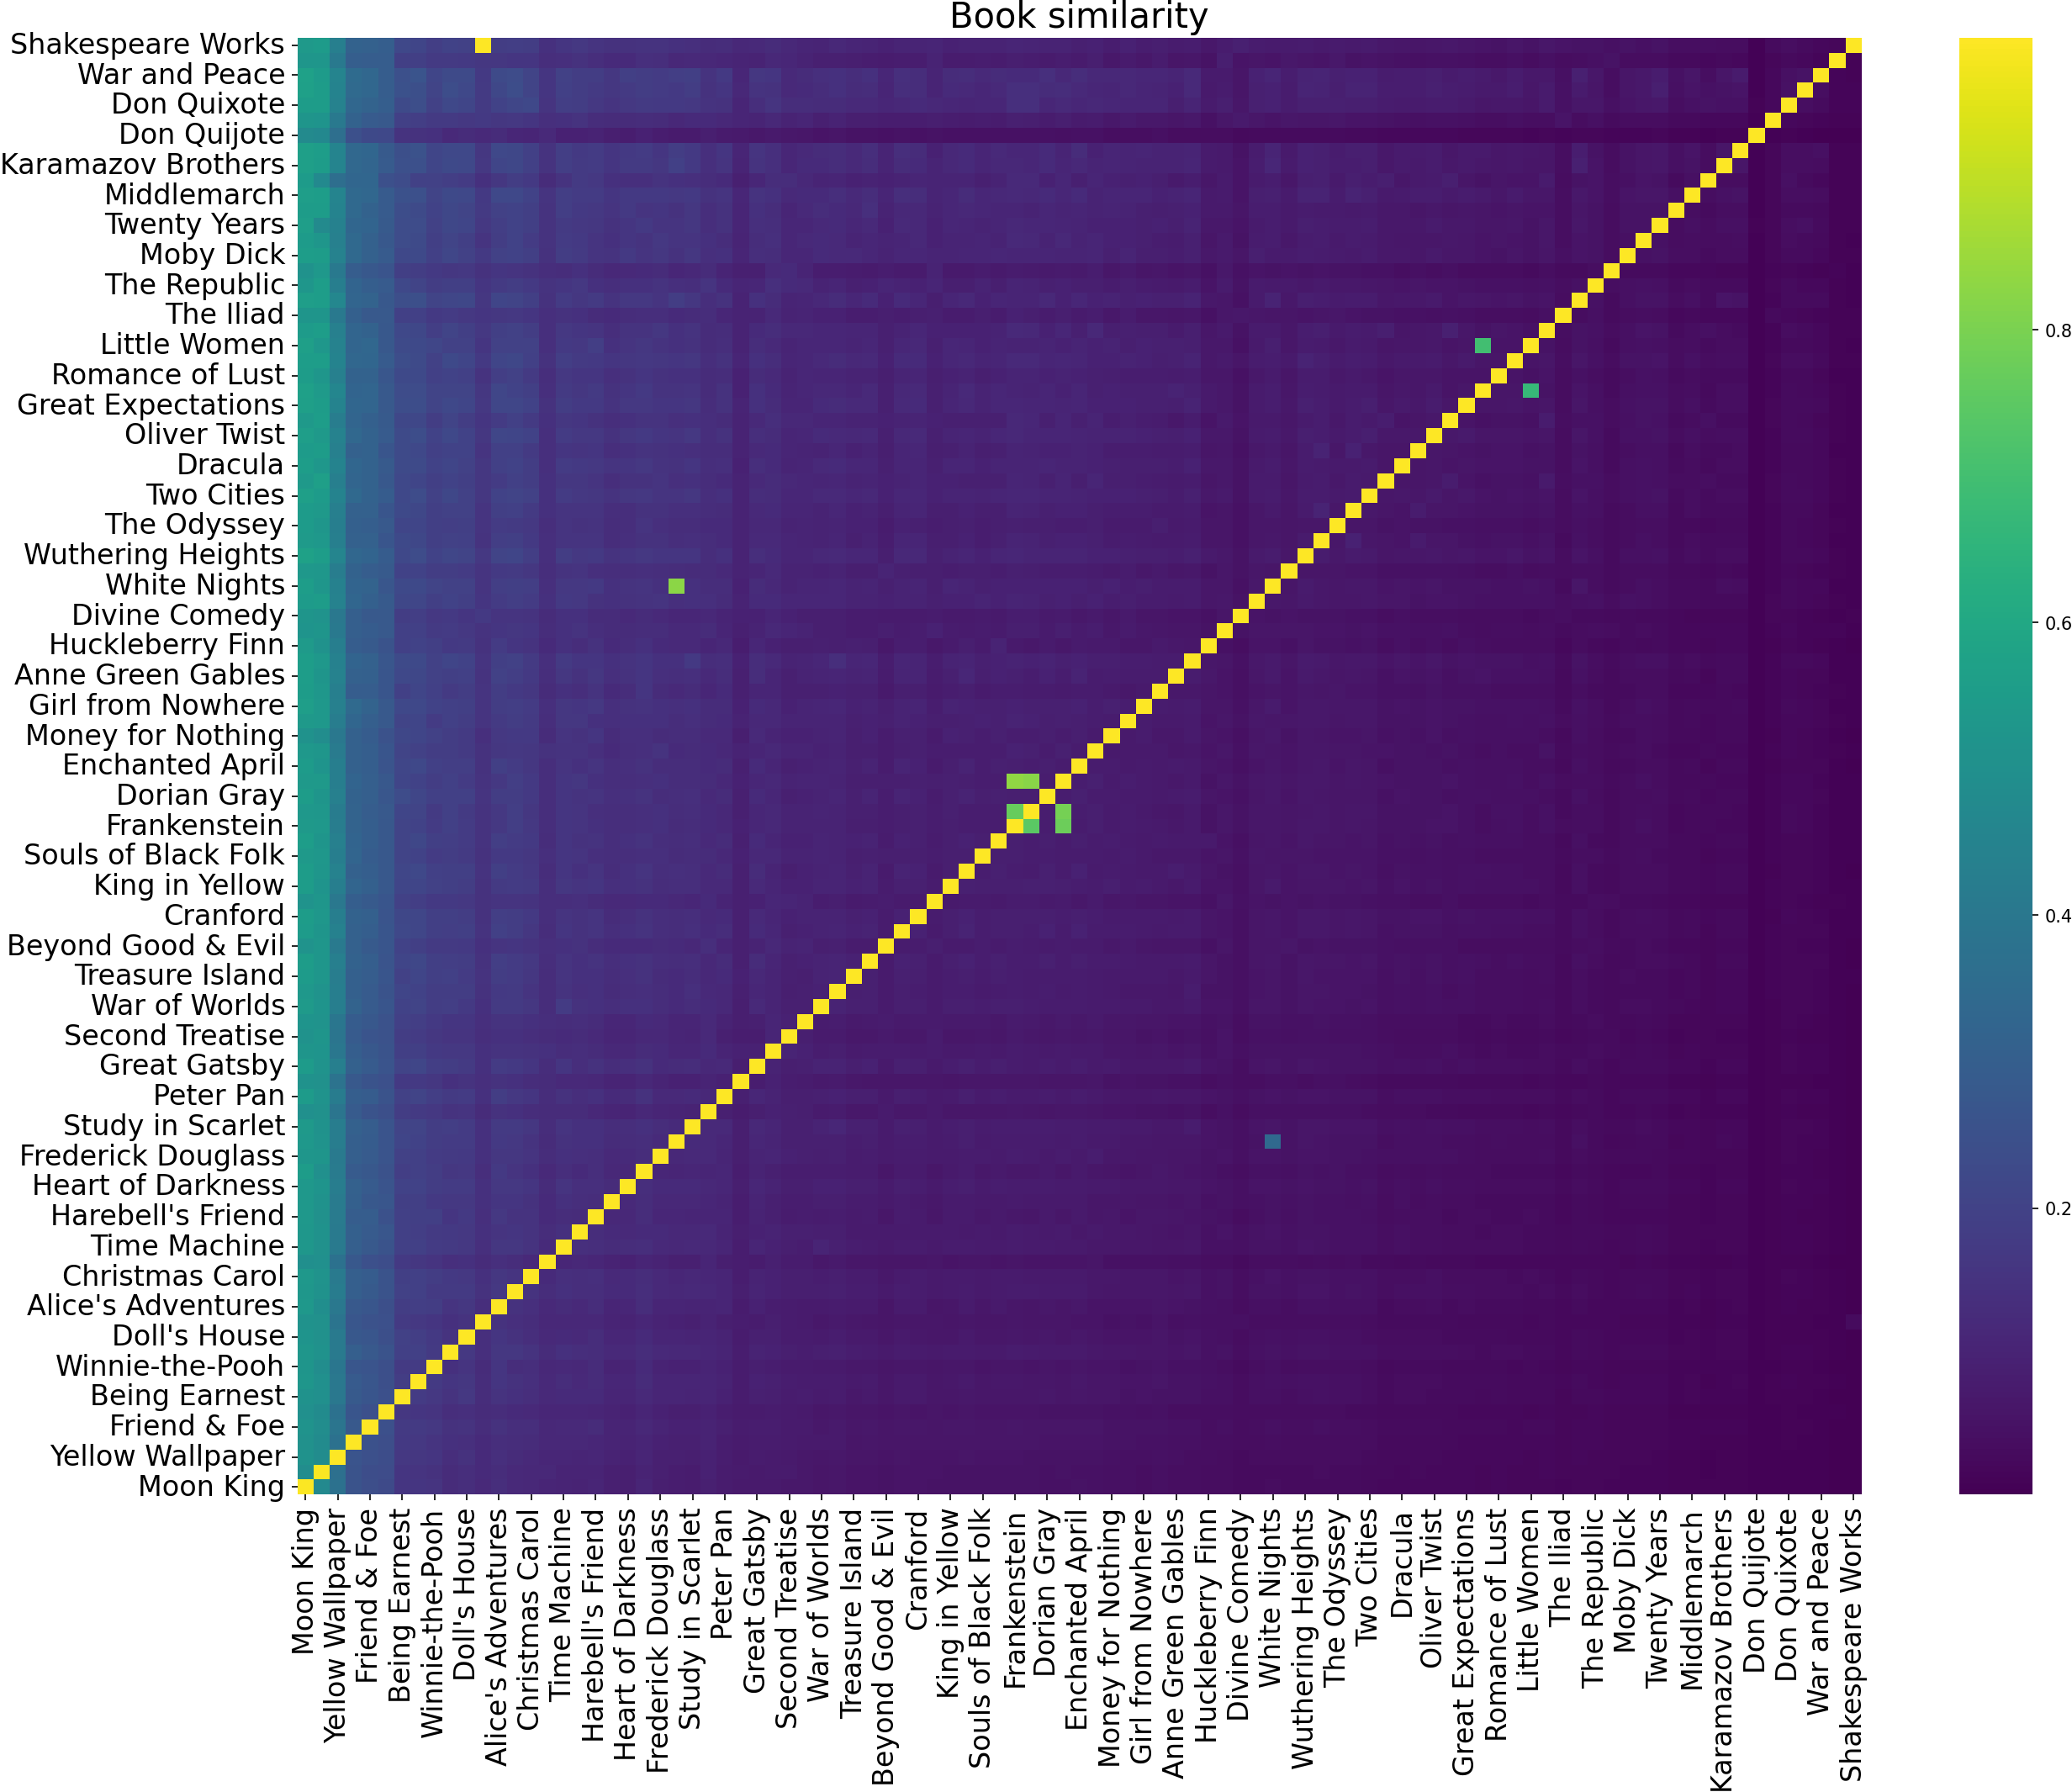
\includegraphics[width=\textwidth]{img/fig_co-compression_file_size.png}
\caption{Similarity scores for pairs of texts. The texts on both axes are sorted by file size.}
\label{fig:heatmap_fsort}
\end{figure}

The similarity score is plotted for pairs of texts in figures \ref{fig:heatmap_ppsort} and \ref{fig:heatmap_fsort}, each plot giving \(x\) on the horizontal axis and \(y\) on the vertical axis, the color of the cell representing \(similarity(x|y)\). In figure \ref{fig:heatmap_ppsort}, the texts on the vertical axis are sorted by how predictive they are on average, and the texts on the horizontal axis are sorted by how predictable they are. In figure \ref{fig:heatmap_fsort}, the same texts are instead sorted by file size on both axes.

The figures were produced using the \texttt{seaborn}, and \texttt{matplotlib} python libraries, and \texttt{pandas} was used to process the data.

The following observations can be made:
\begin{itemize}
  \item In general, larger texts are more predictive.
  \item In general, smaller texts are more predictable.
  \item There are a few very bright dots which do not lie along the diagonal in \ref{fig:heatmap_fsort}. These appear because the dataset includes three versions of Frankenstein which have a high similarity score with each other, as well as the texts for Romeo and Juliet, and the Complete Works of Shakespeare. For this last pair, the latter strongly predicts the first but the first only weakly predicts the second.
  \item There is a strong horizontal dark line in both graphs, which represents a text that is unpredictable regardless of what other text it is paired with. On inspection, this turns out to be Don Quijote, which is in fact unlike the other texts because it is in Spanish, whereas most other texts are in English.
  \item As can be seen in \ref{fig:heatmap_ppsort}, when texts are sorted most-predictive-first on the $y$-axis and most-predictable-first on the $x$-axis, texts generally lie along the diagonal. This indicates that, within a set of texts, there is a trade-off between how predictive a text is and how predictable it is. At least part of this effect has to do with file size, as larger texts tend to contain a larger set of the possible words and expressions of a language.
  \item There is a visible pattern of strong vertical and horizontal lines in \ref{fig:heatmap_fsort} (i.e. there is a low level of noise), indicating that texts tend to be "generally predictive" or "generally predictable" within a given collection.
\end{itemize}

\subsection{Practical application}

As can be seen in the previous figures, it is always the case for any two pairs of texts $x$ and $y$ that "the whole is less than the sum of its parts", i.e. that $C(xy) < C(x) + C(y)$. This opens up the question of whether it is possible to obtain a better compression of $y$ by encoding only that information which it adds to $x$. If this is possible, we should expect that this information should be of the size $C(xy) - C(x)$ which, by the previous equation, is necessarily less than $C(y)$.

Intuitively, this means that if two parties Alice and Bob each have a copy of the works of Shakespeare, and the Alice wants to send over Romeo and Juliet, she can simply encode it by giving the range of pages on which it appears in their shared reference text.

Is this possible to implement in practice? The fact that Lempel-Ziv algorithms work by going through the data in one pass and creating a codebook as they go indicates that $D(xy)$ should contain $D(x)$ as a prefix, where $D(t)$ stands for the compression of $t$. This is, in fact, more or less the case with LZMA, and I was able to create a simple tool that implements this idea, accessible at \url{https://github.com/Guy29/FYP}.

The \texttt{CoCompressor} class I implement is instantiated with two arguments: a reference text $r$ and a compression algorithm. Its \texttt{compress} method takes a text $t$ to compress will output $D(rt)$ with the prefix $D(r)$ removed, and its \texttt{decompress} method takes a text compressed in this way and reverses the process.

Co-compressors instantiated this way differ in their power depending on the choice of reference text. See figure \ref{fig:cocomp_comparison} below for a comparison of the performance of co-compressors trained on different reference texts.

\begin{figure}[h]
\centering
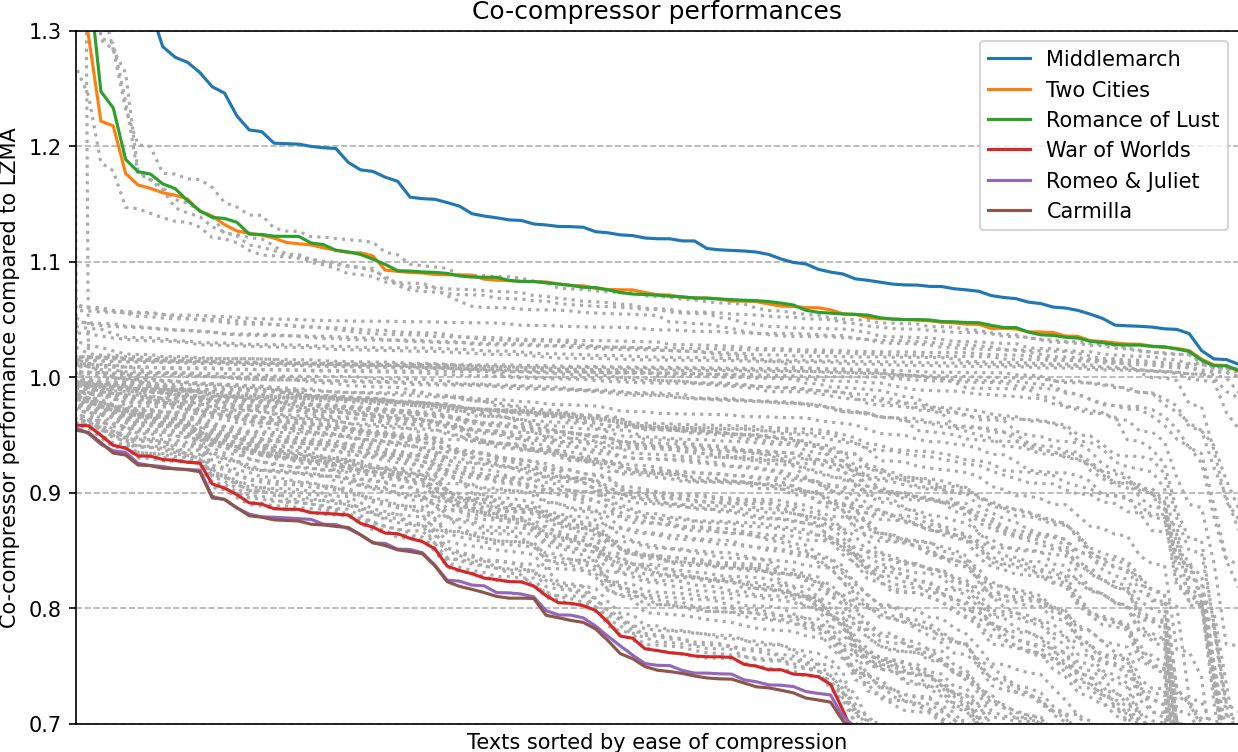
\includegraphics[width=\textwidth]{img/fig_cocomp_performance.png}
\caption{The performance of instances of the \texttt{CoCompressor} class trained on 97 different texts. Each line represents a \texttt{CoCompressor}. The value on the vertical axis is the ratio of the size of the encoding produced by naive LZMA to that produced by the \texttt{CoCompressor}, while the horizontal axis goes through possible inputs for comrpession.}
\label{fig:cocomp_comparison}
\end{figure}

There are a few remarkable things about this figure,

\begin{itemize}
    \item Each co-compressor shows an tan- or sigmoid-like curve, performing exceptionally well on texts which are very similar to it (left side of the plot) and steeply dropping down in performance for sufficiently different texts.
    \item There is very little criss-crossing between the lines in this plot. That is, for any pair of co-compressors, one will usually outperform the other \emph{on every output} in the dataset. Why there should be a strict hierarchy of this sort is not clear, as one might expect that a specific co-compressor would be specialized for one sort of text which are similar to it but not for others.
    \item The best performing co-compressor in this dataset is the one trained on Middlemarch (performing 12\% better than naive LZMA in the median case), followed by A Tale of Two Cities (7.3\%) and The Romance of Lust (7.2\%).
\end{itemize}

It is tempting to explain away the unusual performance of the Middlemarch co-compressor ($CC_{MM}$) as an artifact of the chosen dataset, that it might be situated (historically or otherwise) "in the middle" of the dataset, sharing some features with both preceding and following literary works.

One strong piece of evidence against this is that, as noted above, the performance of co-compressors is strictly hierarchical, and this effect extends all the way to the left of the plot where the co-compressor is fed the text it performs best on (that is, its own text) as its input. Examining this, we notice that

$$CC_{MM}(MM) > CC_t(t) \qquad \forall t \in G$$

where $CC_t(x)$ is the performance of the co-compressor trained on text $t$ when fed input $x$, and $G$ is the dataset. That is, $CC_{MM}$ is not only the most performant co-compressor on all the texts in the dataset, it is also the co-compressor that performs best on its own reference text.

This observation gives a simple way to find other good reference texts for co-compressors: one simply calculates $CC_t(t)$ for each candidate and finds values of $t$ that yield the highest performance.

\section{Natural language compilation}

\section{LLM-based compression}